\documentclass{article}
\documentclass[10pt,a4paper]{report}
\usepackage{tikz}
\usepackage{verbatim}
% not commen package
\usepackage[compact]{titlesec}
\usepackage[hang,flushmargin,stable]{footmisc}
\usepackage[nohyperlinks,nolist]{acronym}
\usepackage[T1]{fontenc}
\usepackage[usenames,dvipsnames,table]{xcolor}
\usepackage{amsfonts,amsmath,amssymb}
\usepackage{array}
\usepackage{booktabs}
\usepackage{csquotes}
\usepackage{enumitem}
\usepackage{eurosym}
\usepackage{fancyhdr}
\usepackage{lastpage}
\usepackage{lineno}
\usepackage{lmodern}
\usepackage{lscape}
\usepackage{makecell}
\usepackage{marginnote}
\usepackage{multirow}
\usepackage{pgfgantt}
\usepackage{pgfplots}
\usepackage{pgfplotstable}
\usepgfplotslibrary{polar}
\pgfplotsset{compat=1.12}
\usepackage{pifont}
\usepackage{sectsty}
\usepackage{sidecap}
\usepackage{soul} % for smarter (word-wrapping) underlining
\setul{1pt}{.4pt} % 1pt below contents
\usepackage{wrapfig}
\usepackage{xspace}
\usepackage{forest}
\usepackage{tikz}
\usetikzlibrary{arrows,shapes,chains}
\usepackage{hyperref}
\hypersetup{hypertex=true,
            colorlinks=true,
            linkcolor=blue,
            anchorcolor=blue,
            citecolor=blue}

% commen package
\usepackage{fancyhdr}
\usepackage{setspace}
\usepackage[utf8]{inputenc}
\usepackage{multirow}
\usepackage{subcaption}
\usepackage{enumitem}
\usepackage{listings}
\usepackage{float}
\usepackage{graphicx}
\usepackage{geometry}
\geometry{left=2.0cm,right=2.0cm,top=3.0cm,bottom=2.0cm}
\usepackage{times}
\usepackage{mathptmx}
\usepackage{color}
\usepackage[dvipsnames]{xcolor}
% HotFix from http://tex.stackexchange.com/a/300259/84485
% Version1 of titlesec is not compatible with the latest texlive. 
% Either the titlesec package must be updated, or the following HotFix used:
\usepackage{etoolbox}
\makeatletter
\patchcmd{\ttlh@hang}{\parindent\z@}{\parindent\z@\leavevmode}{}{}
\patchcmd{\ttlh@hang}{\noindent}{}{}{}
\makeatother

% Fonts
\usepackage{libertine}
\usepackage[scaled=.875]{gillius2}
\usepackage[libertine]{newtxmath}

% Size
\headheight=20pt
\setlength{\parindent}{0pt}
\titleformat*{\section}{\bold\Huge}
\titleformat*{\subsection}{\huge}
\titleformat*{\subsubsection}{\large}
\renewcommand{\headrulewidth}{0pt}
\renewcommand{\baselinestretch}{1.0} 

% Color
\definecolor{royalblue}{rgb}{0.0, 0.14, 0.4}
\allsectionsfont{\sffamily\bfseries\raggedright\color{royalblue}}
\let\oldfootnotesize\footnotesize
\newcommand{\highlight}[1]{\colorbox{gray!15}{\small{#1}}}
\newcommand{\marginLeft}[1]{\reversemarginpar\marginnote{\rotatebox{90}{\sffamily\bfseries\color{royalblue}\large{\phantom{j}#1}}}}
\newcommand{\marginRight}[1]{\normalmarginpar\hspace{0pt}\marginpar{\rotatebox{0}{\sffamily\color{gray}\normalsize{#1}}}}
\newcommand\colorrule{\vspace{4px}{\color{lightgray}\hrule}\vspace{4px}}

% Bibliography
%\bibliography{bibliography}
%\usepackage[style=chem-acs,doi=false]{biblatex}

% Headers and Footers
\renewcommand{\footnotesize}{\fontsize{10bp}{1em}\selectfont}
\renewcommand{\cite}{\autocite} % citations in footnotes
% Explicitly set footnote font size to match call (i.e., 8pt).
% Taken from http://tex.stackexchange.com/a/249422/84485
\makeatletter
\renewcommand\footnotesize{%
   \@setfontsize\footnotesize\@ixpt{8}%
   \abovedisplayskip 8\p@ \@plus2\p@ \@minus4\p@
   \abovedisplayshortskip \z@ \@plus\p@
   \belowdisplayshortskip 4\p@ \@plus2\p@ \@minus2\p@
   \def\@listi{\leftmargin\leftmargini
               \topsep 4\p@ \@plus2\p@ \@minus2\p@
               \parsep 2\p@ \@plus\p@ \@minus\p@
               \itemsep \parsep}%
   \belowdisplayskip \abovedisplayskip
}
\makeatother


\usepackage{color}
\definecolor{dkgreen}{rgb}{0,0.6,0}
\definecolor{gray}{rgb}{0.5,0.5,0.5}
\definecolor{mauve}{rgb}{0.58,0,0.82}


\lstdefinestyle{myPython}{% myPython是格式的名字
	frame = lrtb, % 显示边框
	captionpos=t, % 代码呈现的位置
	breaklines=true,%自动换行
	columns=fixed,  %
	%如果不加这一句,字间距就不固定,很丑,必须加
    basewidth=0.5em,
    showstringspaces=false,
    showspaces=false,
    flexiblecolumns,
	language=Python,
	aboveskip=3mm,
	belowskip=3mm,
	showstringspaces=false,
	columns=flexible,
	numberstyle=\small\color{red},
	basicstyle={\Monaco},
	keywordstyle={\color{blue}\Monaco},
	commentstyle={\color{dkgreen}\Monaco},
	stringstyle={\color{mauve}\Monaco},
	breaklines=true,
	breakatwhitespace=true,
	tabsize=3
}


\definecolor{codegreen}{rgb}{0,0.6,0}
\definecolor{codegray}{rgb}{0.5,0.5,0.5}
\definecolor{codepurple}{HTML}{C42043}
\definecolor{backcolour}{HTML}{F2F2F2}
\lstdefinestyle{MySQL}{
    language        =   SQL, % 语言选Python
    basicstyle      =   \Monaco,
    % numberstyle     =   \ttfamily,
    keywordstyle    =   \color{blue}\Monaco,
    keywordstyle    =   [2] \color{teal},
    stringstyle     =   \color{magenta},
    commentstyle    =   \color{red}\ttfamily,
    breaklines      =   true,   % 自动换行,建议不要写太长的行
    columns         =   fixed,  % 如果不加这一句,字间距就不固定,很丑,必须加
    basewidth       =   0.5em,
}
\lstset{
    basicstyle          =   \Monaco,          % 基本代码风格
    keywordstyle        =   \fontspec{Monaco},          % 关键字风格
    commentstyle        =   \rmfamily\itshape,  % 注释的风格,斜体
    stringstyle         =   \ttfamily,  % 字符串风格
    flexiblecolumns,                % 别问为什么,加上这个
    % numbers             =   left,   % 行号的位置在左边
    showspaces          =   false,  % 是否显示空格,显示了有点乱,所以不现实了
    numberstyle         =   \ttfamily,    % 行号的样式,小五号,tt等宽字体
    showstringspaces    =   false,
    captionpos          =   t,      % 这段代码的名字所呈现的位置,t指的是top上面
    frame               =   lrtb,   % 显示边框
    style = MySQL
}




\def\BibTeX{{\rm B\kern-.05em{\sc i\kern-.025em b}\kern-.08em
    T\kern-.1667em\lower.7ex\hbox{E}\kern-.125emX}}
\usepackage{cite}


\pagestyle{fancy}                   % 设置页眉页脚
\lhead{DATA70202}   %页眉左侧显示页数                 
% \chead{}                                  %页眉中
\rhead{Group 10}                         %章节信息                       
\cfoot{\thepage}      
\usepackage[utf8]{inputenc}

\begin{document}
\setlength{\baselineskip}{20pt}%行间距
\setlength{\parskip}{5pt}
\title{\Huge Apply Data Science Project Report \\[1cm]
        \bf\LARGE DATA70202 }
\author{\Large Jiazheng Wen\\ 10854686 \\[10pt]
                Ziyan Wang \\ 10653294 \\[10pt]
                Zida Zhou \\ 10956712 \\}
\date{\Large \today}

\makeatletter
    \begin{titlepage}
        \begin{center}
	        {
\includegraphics[width=12cm]{Settings/TitlePicture.png}}
	   {\ \\}
        \vbox{}\vspace{3cm}
            {\@title }\\[1cm] 
            {\@author}\\[15pt]
            {\@date}\\[20pt]
            {\Large Total Word Count: \bf 2603 \\ \ \\}
        \end{center}
    \end{titlepage}
\makeatother

\section*{Introduction}
To make land use design and planning more rational, a new type of design concept has been proposed: Geodesign. It combines digital technology with traditional geographic information systems, aiming to provide more analysis and decision-making options based on data visualisation \cite{bib1}. Meanwhile, the implementation of this concept requires specific tools to help, such as high-level programming languages, large data storage support and hardware that supports high concurrency and computing \cite{bib2}. The emergence of Geodesignhub opens up a new world for urban design and geographic data analysis. It not only inherits the essence of Geodesign, but also simplify the process of solving geographical-related problems and customize solutions for different practical situations \cite{bib3}. However, Geodesignhub is not omnipotent: It excels only in simple geographic data calculation computation, data migration and application, and visualization, but is powerless in complex data-analysis problems. For example, the software cannot directly calculate the similarity of the two areas, nor can it tell by name whether they are of the same type (residential land, school land or factory land). In this project, the functionality of Geodesignhub was extended using computer languages to perform deeper analysis of geographical data, such as geographic area similarity, semantic similarity of geographic area names. 

\marginLeft{}
The flow of the whole project was extremely well designed and performed. At the beginning, two design patterns were provided as the project's data sources. Several key features, which can be divided into textual features and numerical features, were extracted from these data sources. Text features include tags, labels, descriptions while numerical features are two-dimensional coordinate tuples containing latitude and longitude. Then, the similarity of the two design patterns in different focuses was analysed based these features. A set of matrices of similarity across four parameters was designed to measure the similarity: Taxonomy, Topology, Geography, Conceptual. In order to better judge the degree of compliance of each parameter, a five-level indicator was introduced: 
"low similarity" was represented by number 1 and "high similarity" was represented by number 5.  Finally, the results of the experiments were sublimated and visualised so that these results can be used as direct indicators to facilitate rational decision-making process.

\marginLeft{}
This report is organized as follows: First, a literature review of the geographical analysis and related studies is given to find suitable investigation methods and experimental models. Then, basic data processing methods are introduced. After that, different algorithm flows are designed for different similarity parameters. Moreover, the comparison of indicators on the four parameters is performed. Lastly, reflections on the practicality and generalization of the algorithms are discussed in the conclusion.  

\section*{Literature Review}
In urban planning, the development of design proposals is a fundamental aspect. It is a common problem in planning that design proposals are too subjective or controversial. In order to avoid it, the bill \textit{the Planning and Compulsory Purchase Act, 2004}, requires planners to submit a Design and Access Statement (DAS) with most applications. Paterson\cite{bib4} investigated whether the introduction of DAS was helping the design decision making process, using primary data from the north-east of England. The findings showed that DAS was useful but limited. More interactive communication and design for sustainability in the design process are desirable.

Recently, strengthening the links between planners and communities has become an important topic in planning. Gordon and Manosevitch\cite{bib5} introduced the concept of augmented deliberation and demonstrated its implementation in a pilot project. Designers and the local community gathered in a physical space and a virtual space simultaneously to discuss the design, enabling productive and meaningful public deliberation. Their research has demonstrated that this approach enhances the ability of non-specialist participants to understand the space, thus enabling the creation and sharing of local experiences and facilitating effective public deliberation. However, such an approach requires significant financial, technical, and physical resources which may not be feasible for all communities at all times.

Various aspects of planning can be complex processes. For example, for transport planning decisions to be stable, transparent and participatory, they need to be well-structured and use quantitative analysis from the fields of engineering and economics.\cite{bib6}

GIS (Geographic Information System) has been gradually introduced into the planning field in recent years, providing planners with a variety of convenient functions.\cite{bib7} GIS is an operational and affordable planning information system. It is increasingly becoming an important component of planning support systems. Recent advances in the integration of GIS with planning models, visualization and the Internet will make GIS even more useful for planning. GIS can be applied at all stages of urban planning, enabling functions such as data management, visualization, spatial analysis, and modelling components of GIS varies.

Based on a state-of-the-art study and a thematic analysis of 114 articles, published in 2004–2014 and found through snowball sampling, Billger, Thuvander and Wästberg\cite{bib8} discussed the development and implementation of digital visualization tools for dialogue in planning. A wide range of examples of visualization tools for dialogue has been found; either based on 2D maps, 3D environments or gaming. There is a tendency for the usability studies to have gone from experimental and prototype studies to more and more concern real planning processes and implementation. Challenges are related to integration of qualitative and quantitative data, representation of data as regard appropriate levels of realism and detailing, as well as the user’s experience and the appearance of the digital models.

 Natural Language Processing (NLP) has shown potential as a promising tool for harnessing underutilized urban data sources\cite{bib9}. The application of NLP to the study of urban design is still in its infancy. Current applications fall into five areas: urban governance and management, public health, land use and functional areas, mobility and urban design. By mining the application of NLP in urban planning, it can be of great help to decision makers.


\section* {Methodology}
\subsection* {Data Set}
The whole project is based on two design patterns, including calculations, comparisons. And the dataset used in this project, written in json format, is a concrete representation of the design pattern. json uses attribute-pairs and arrays to store and transmit data objects for human reading(WIKI-https://en.wikipedia.org/wiki/JSON). The basic structure of the JSON file shown in Picture 1:

\begin{figure}[H]
\caption{The Basic Structure for the Json files}
\centering
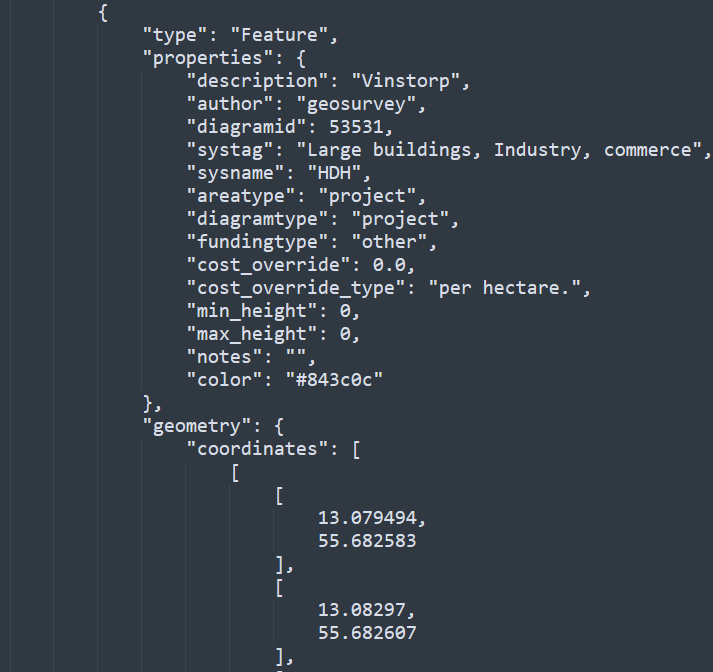
\includegraphics[scale=0.5]{pic1.png}
\label{fig:label}
\end{figure}
A json file may have multiple structures as shown, each representing a polygon or line segment in the map. Only the sysname, description attributes and geometry arrays are required for a project in a structure. The sysname represents the use of an area, of which there are eight. Description is a deeper representation of the area. Geometry stores the overall latitude and longitude array of the region.




\subsection*{Data Pre-processing and EDA}
The main objectives for pre-processing stage is converting JSON (unstructured) data to structured format and finding the underlying metadata.
\par
For obtaining structured data and its metadata, Python is used for reading and manipulating the JSON files for two designs. With the aid of library json, the two GEOJSON files can be stored as dictionary in Python. After that, by investigating the data, some rudimentary rules can be found:
\par
(1) Both of the JSON files share the same hierarchical structure.
\par
(2) The structure can be simplfied to two layers and the outer layer of each JSON is a list, which contains multiple objects.
\par
(3) The objectives in inner layer also feature similar structures, that is, most of the attributes of the objects is common.
\par
To map GEOJSON data to urban desgin or planning in real world, it is apparent that the JSON file itself refers to the entire design. And a design consists several entities, such as a land for housing, a place for building a park or an express way, which can be mapped to the objects in the inner layer of JSON data. Also, the detailed information of each entity is corresponded to the values of attributes of each object. It can be seen that the relationship between GEOJSON data and its physical meaning can facilitate the process of data transforming and metadata retrieving.
\par
The next step is to investigate the attributes of each entity. First, it is obvious that the attributes can be divided into numerical and textual attributes. The numerical attributes define the geometric feature of the entity while the textual attributes clarify the label, description and annotation of the design.
\par
For numerical attributes, the first attribute is ID, which is the identifier of each entities. The most important feature is geographical coordinates, which determines the location of an entity. Also, other features like area, length can be derived from this attribute. Other attributes like minimum/maximum height and cost override are all the same amongst the entities. Thus, those features will be reduced. The last attribute is colour and it can only influence the readability of the images of a design generated by GEOJSON tool but has no contribute to the semantic of the design. As a result, attribute color will also be erased.
\par
For textual attributes, the first useful one is type. Attribute type can be only set to ``Polygon" and ``LineString", which indicates that whether the entity is of a closed figure or line. Different kinds of shape also require different method for manipulating coordinates. The second attribute is description. This feature is important since it tells the semantic of each entity, for example, an entity with description ``Bike highway" can be directly understood as a kind of road exclusively for bicycles. Another attribute is ``systag", which assigns each entity with a geodesignhub built-in label. The value of this attribute can only be ``Large buildings, Industry, commerce", ``Small buildings, low density housing", ``Agriculture, Forestry" or ``Roads, transport". It is attribute ``systag" that has divided the entities into four categories roughly. 
\par
After sorting numerical and textual features, the metadata can be obtained and Table 1 illustrates the attributes that will be used and their comments.
\begin{table}[H]
\centering
\caption{The parameters for the example}
\label{tab:my-table}
\begin{tabular}{|c|c|c|}
\hline
NAME & TYPE & DESCRIPTION \\ \hline
id & INT & The identifier \\ \hline
coordinate & (FLOAT, FLOAT) & Geographical location of a vertex \\ \hline
description & TEXT & Description of each entity \\ \hline
systag & TEXT & Can only be four values. \\ \hline
\end{tabular}
\end{table}
After obtaining metadata from the two designs of urban planning, the manipulation against the data can be executed under the guidance of metadata.
\subsection*{Taxonomy----wzy}
1. 我们根据sysnmae去判断same idea。。。。 sysname完全相同: sysname完全相同就叫same idea 4级,description,不是相似,4级,是相似5级。snameidea, descriotion   333.3一级,判断
The similarity of taxonomy with regard to the designs is that the locations and places can be categorised into the same group. A very direct example is that a place for ``school" and an area that is projected to be a ``campus" can be naturally grouped together. The reason is that both of them represents the same idea. Although the two schools may be situated in very different places, can be designed for different area, they both stand for education institutes and are obviously not identical to places with other idea like ``industrial plants".
\par
It can be found that finding taxonomy similarity mainly focuses on the description, comments or labels of each figure in the designs and can neglect other geometric attributes. That is, the textual attributes in the design is the key for defining taxonomy similarity and therefore, natural language process (NLP) and text mining methodology can be exploited for obtaining similarity of taxonomy.
\par
From the perspective of text mining, it can be seen that the similarity of taxonomy against textual information is to gather the text with same meaning into groups, which can be also regraded as finding synonyms. In other words, the problem of finding latent taxonomy similarity in the two designs can be solved by finding the similarity of the textual attributes of each design using NLP algorithm.
\par
Since the textual information of each shape in the designs are stored in attribute Description and hence, the description of each figure is utilise for finding taxonomy similarity using NLP approaches. 

实体(entity),包括线和多边形,把shape换成entity?


The core idea for finding taxonomy similarity between descriptions is to convert them into word vectors and thereby the distance between the vectors can be computed, where the distance is directly correlated to similarity of taxonomy.
\par
In terms of the method of embedding descriptions into vectors, Global Vectors for Word Representation algorithm (GloVe) is adopted. GloVe is an unsupervised learning method based on word count based and overall statistics, which can capture the latent analogy and synonym between words \cite{pennington2014glove}. After obtaining word vectors, the description can be embedded into a vector by adding the vector of its words. The following formula shows the process of embedding description into vectors:
$${\rm vec}(d)=\sum_{i=1}^{n}{\rm vec}(w_i)$$
where $d$ is a description of a figure and it is composed by words $w_1,w_2,...,w_n$.
\par
For the metric of distance between vectors, the cosine similarity is used, which can expressed by the following formula:
$$s={\rm cos}(\theta)=\frac{|v_1\cdot v_2|}{||v_1||||v_2||}$$
where $s$ is similarity and $v_1$,$v_2$ are the vectors for two descriptions. The value of cosine similarity is corresponding the taxonomy similarity and if the value is closer to 1, then the two descriptions are very similar, otherwise, they hardly have the same idea. 
\par
By inputting the textual data of the given geojson files, the taxonomy similarity can be visualised by the following heat map.
\par
It can be found that the designs with the same descriptions definitely feature maximum similarity for taxonomy, for example, New Housing. And the descriptions with similar meanings also achieves high similarity like Bike Lane and Bike Path. Besides, the designs with irrelevant textual attributes, such as New River and Bike Highway, display less similarity score, which is also not out of expectation in real world. 
\subsection*{Topology---zhouzida}
In addition to the textual attributes, the main difference between the designs is located in the geometric attributes. This project uses the json file outputted from QGIS as the dataset, where the main geometric attribute is the coordinates attribute. Coordinates are the set of latitude and longitude of multiple corner points. The entities in the design scheme are lines (roads) and polygons (areas). (Whether an entity is a road or an area can be judged by determining whether the start and end points of each entity's "coordinates property" are the same.)

Topological similarity is defined as the similarity of different geometry for the same place. In practical planning work, for practical purposes and due to various factors, entities are often designed as irregular polygons or folds. Therefore, a comparison of the similarity of entities in geometry should focus on the ratio of the overlapping area of the same places in the two scenarios to the total area of the planned area. The following part of this section focuses the derivation and presentation of the algorithm on polygons.
(要讨论:要不要研究线?我们要怎样去认为两条线是一样的?比如说某条折线的某段直线,必须完全重合才认为一样?如果斜率和长度一样,坐标偏移了一点点,能认为是一样吗?能简单和多边形类比吗?)

The main challenge of this part of the work is to derive a method for calculating the area of a polygon when the coordinates of the corner points of the polygon are known. The derivation starts with the simplest polygon, the triangle, and is then extended a method for calculating the area that can be applied to all general polygons.

Calculation using matrix determinants is at the heart of this part of the algorithm. The geometric meaning of a matrix determinant is the directed area of a parallelogram with two vectors as a set of neighbors. (Directed in the sense that the area is positive if the second vector is rotated 0 to 180° counterclockwise with respect to the first vector, and negative if the second vector is rotated 0 to 180° clockwise with respect to the first vector.)

Suppose there is a general triangle and we set up a rectangular coordinate system to place this triangle in it. First, we assume that the origin O lies inside the triangle (the case where the origin is outside the triangle will be described later).

\begin{figure}[H]
\caption{$\triangle ABC$ in The Coordinate System}
\centering
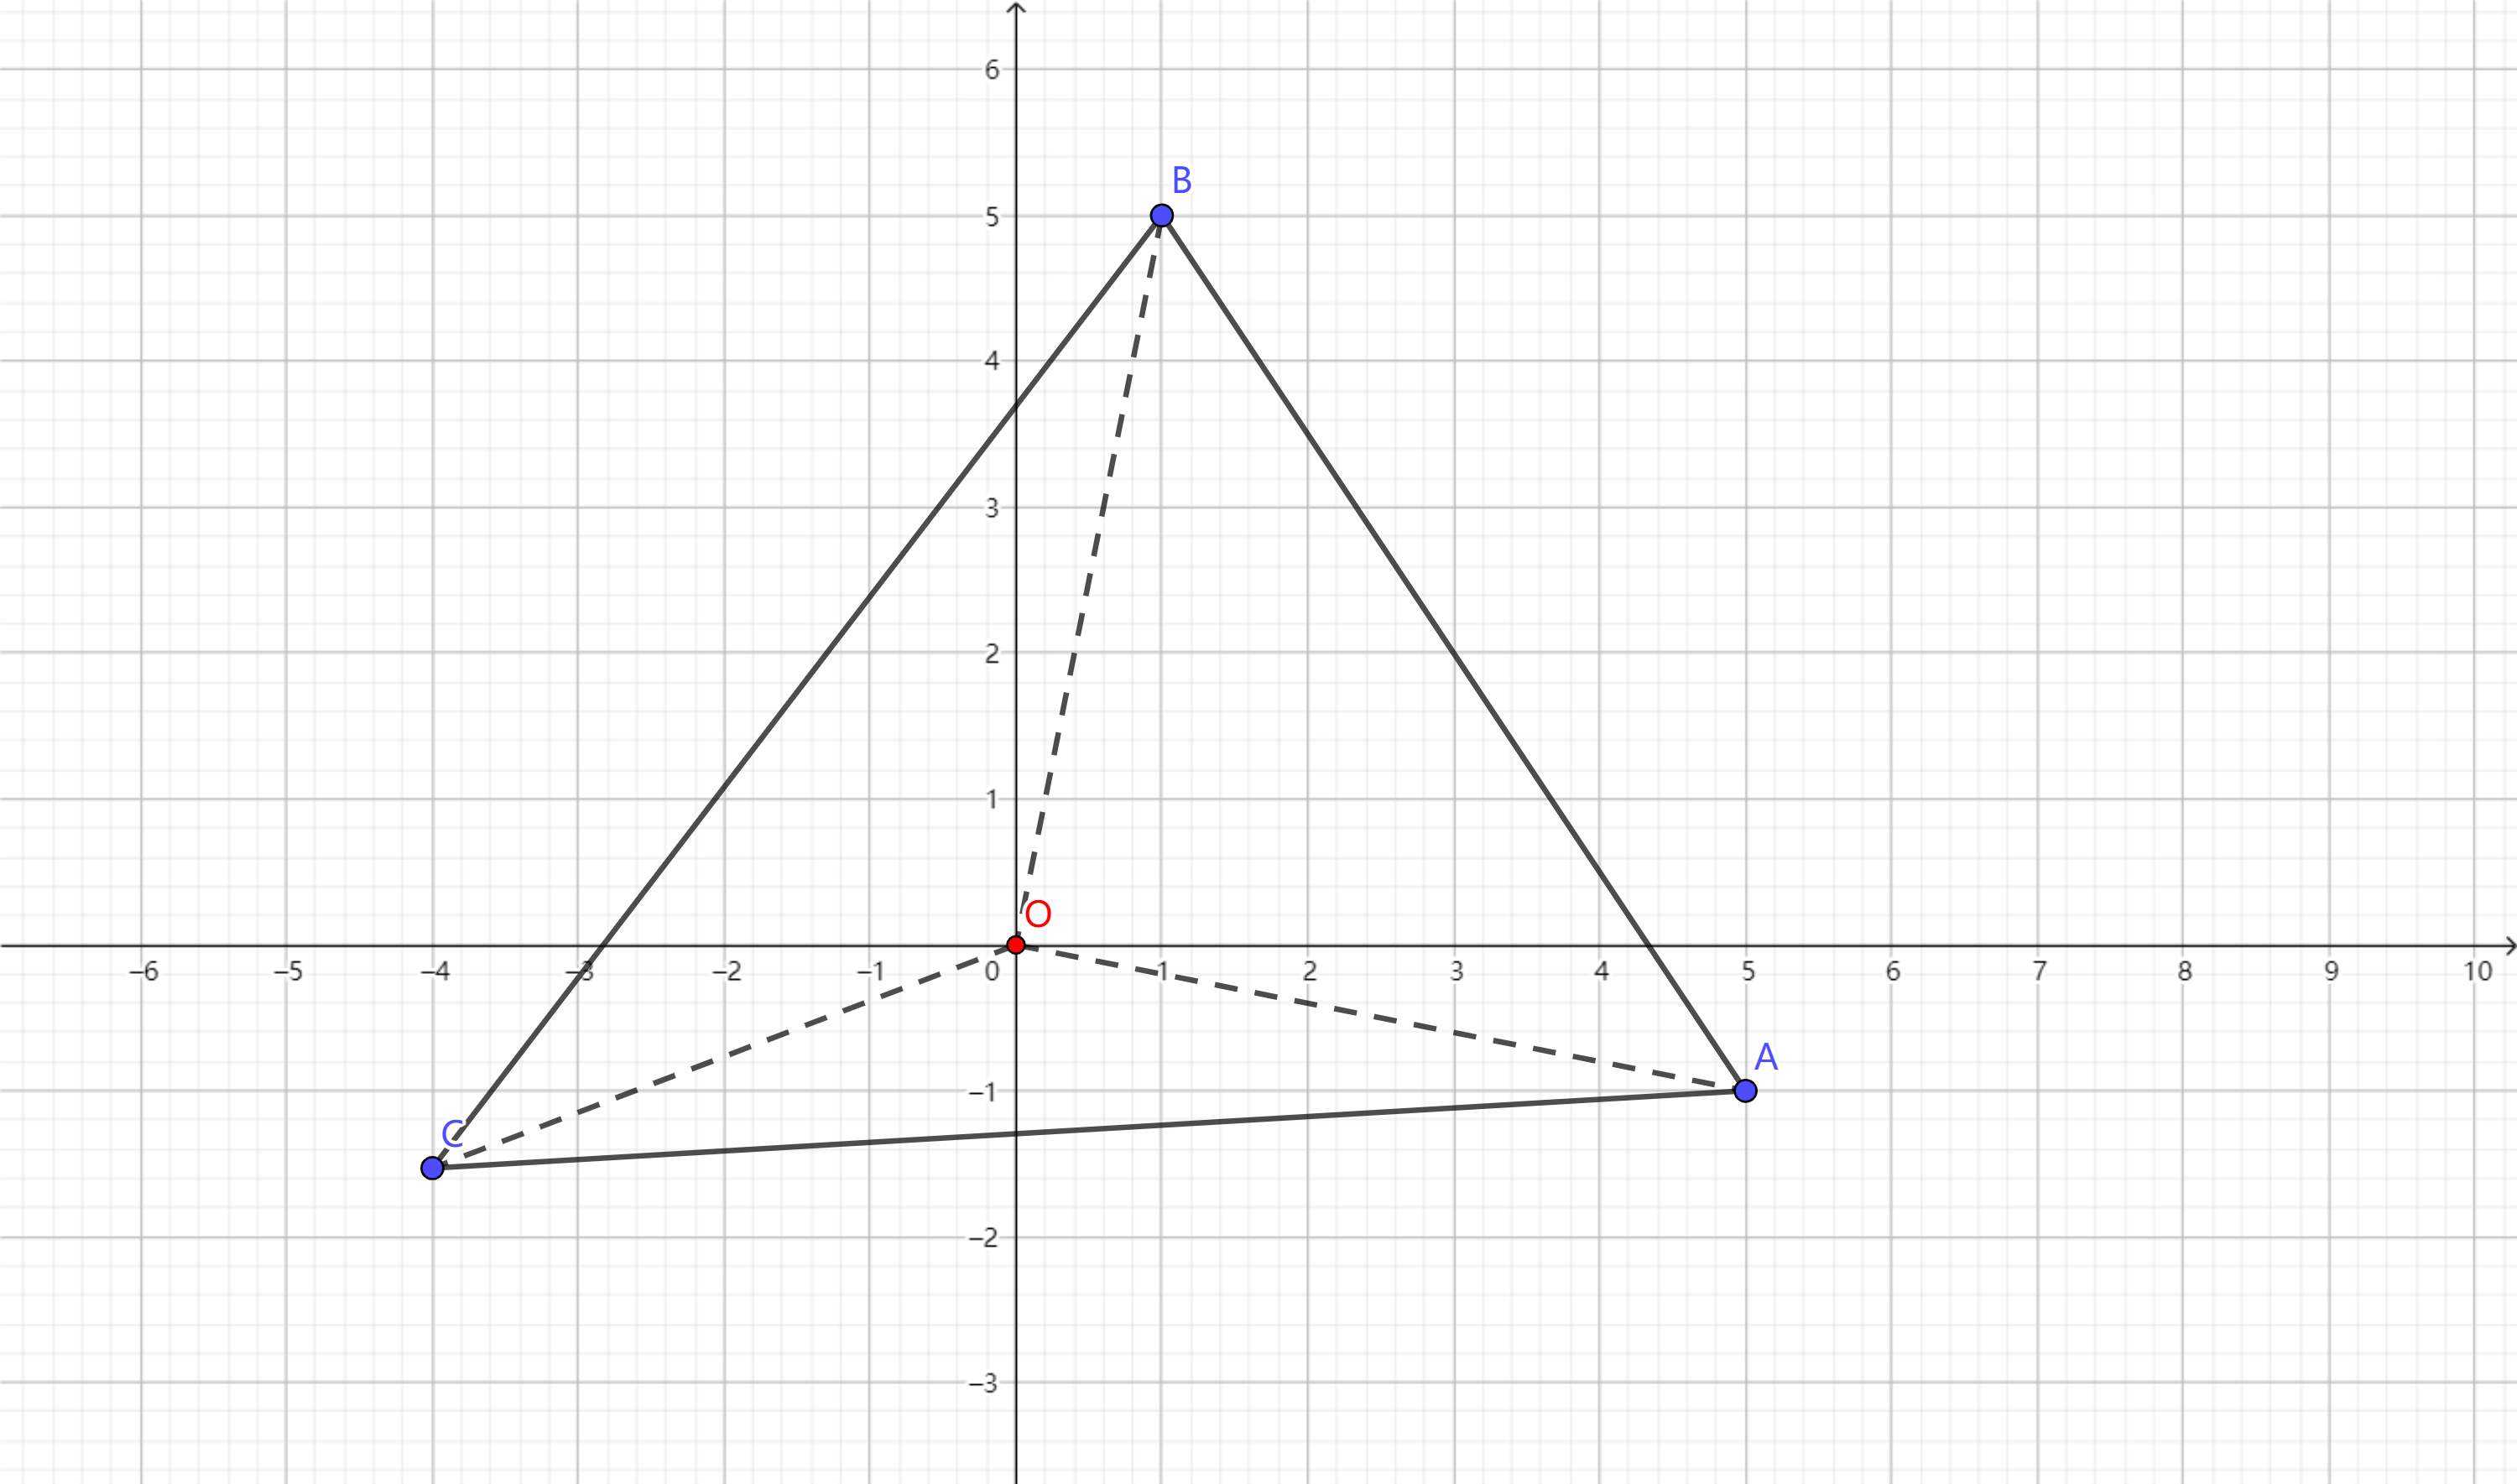
\includegraphics[scale=0.5]{pic2.png}
\label{fig:label}
\end{figure}

Then $S_{\triangle ABC}$ is split into $S_{\triangle AOB}$, $S_{\triangle AOC}$ and $S_{\triangle BOC}$. Let’s focus first on one of these, $S_{\triangle AOB}$.

\begin{figure}[H]
\caption{Flipping $\triangle ABC$}
\centering
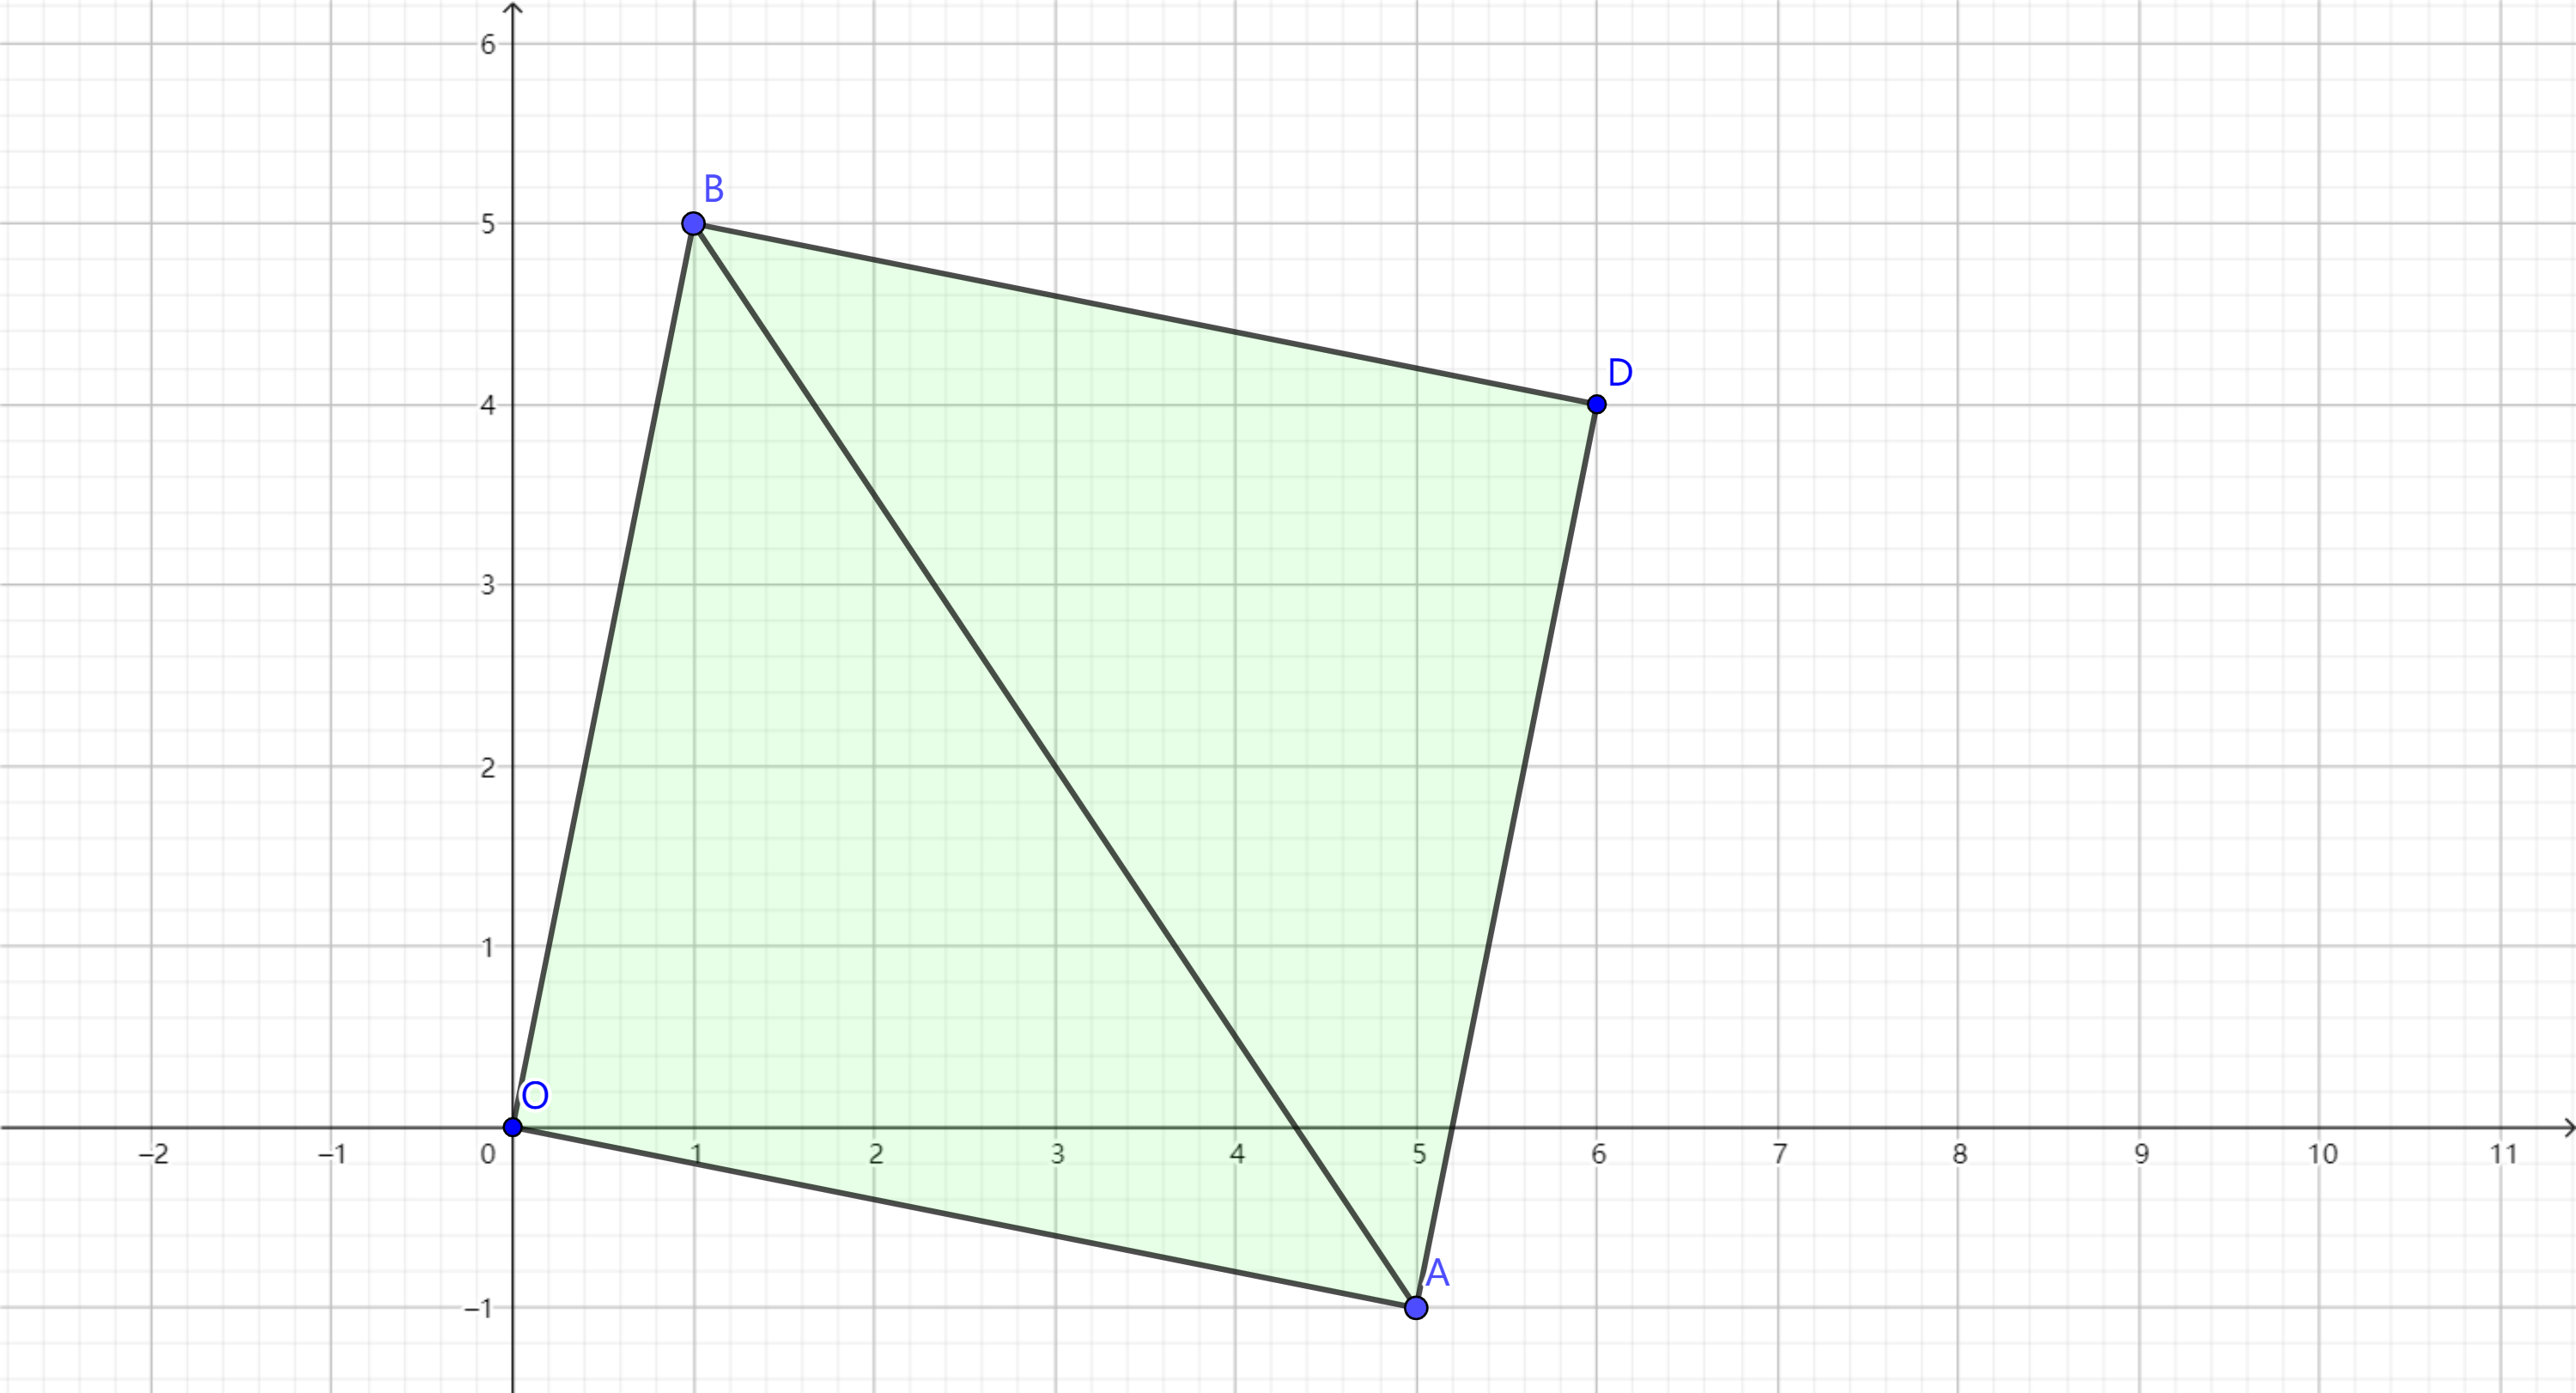
\includegraphics[scale=0.5]{pic3.png}
\label{fig:label}
\end{figure}

Taking AB as the axis of symmetry and flipping $S_{\triangle ABC}$, the area of parallelogram AOBD can be expressed in matrix determinant as:

\begin{equation}
\begin{split}
S_{\parallelogram AOBD}=\begin{vmatrix}
  x_{A} &x_{B}  \\
  y_{A} &y_{B} 
\end{vmatrix}
\end{split}
\end{equation}

So that the area of $\triangle AOB$ is half of it;

\begin{equation}
\begin{split}
S_{\triangle ABC} =\frac{\begin{vmatrix}
  x_{A} &x_{B}  \\
  y_{A} &y_{B} 
\end{vmatrix}}{2}=x_{A}y_{B}-x_{B}y_{A}  
\end{split}
\end{equation}

The area of $\triangle AOC$ and $\triangle BOC$ is calculated in the same way, and then we get:

\begin{equation}
\begin{split}
S_{\triangle ABC}
&=S_{\triangle AOB}+S_{\triangle BOC}+S_{\triangle COA}\\
&=\frac{\begin{vmatrix}
  x_{A} &x_{B}  \\
  y_{A} &y_{B} 
\end{vmatrix}+\begin{vmatrix}
  x_{B}& x_{C}\\
  y_{B}&y_{C}
\end{vmatrix}+\begin{vmatrix}
  x_{C}&x_{A} \\
  y_{C}&y_{A}
\end{vmatrix}}{2}\\
&=\frac{(x_{A}y_{B}-x_{B}y_{A})+(x_{B}y_{C}-x_{C}y_{B}) +(x_{C}y_{A}-x_{A}y_{C})  }{2}\\
&=\frac{(x_{A}y_{B}+x_{B}y_{C}+x_{C}y_{A})-(x_{B}y_{A}+x_{C}y_{B}+x_{A}y_{C})}{2}
\end{split}
\end{equation}

When the origin O is outside $\triangle ABC$, there will be a sub-triangle whose area determinant is negative, so the formula still applies when brought into $\triangle ABC$.

This area calculation method can be extended to any polygon. Given a general polygon, it can be divided into multiple triangles. The area of the polygon can be obtained by summing the areas of these triangles using the matrix determinant.
The formula is:
\begin{equation}
\begin{split}
S_{Polygon}= \left | \frac{(x_{1}y_{2} +x_{2}y_{3}+...+x_{n}y_{1} )-(x_{1}y_{n} +x_{2}y_{1}+...+x_{n}y_{n-1})}{2}  \right | 
\end{split}
\end{equation}

where i=1,2,...,n denotes the i-th point and ($x_{i}$, $y_{i}$) denotes the coordinates of the i-th point.

After discussing how to calculate the area of a polygon using corner point coordinates, the next step is to discuss the calculation of topological similarity.

Suppose there are two planning designs to compare, D1 and D2, and the sites they are planning to develop are called Area1 and Area2, with areas S1 and S2 respectively, and the area planned to be developed in both schemes is called Overlapping Area, which has an area of S3.

It should be noted that the area S3 of the overlapping area between the two proposals requires a solution algorithm to be devised. It is a typical problem of solving for the intersection of polygons and has some computational complexity. We have designed the  solution algorithm to calculate the intersection of polygons.Its proof process is very cumbersome, so here we will directly give the concepts required by the algorithm and some properties used by the algorithm.
The specific relevant proof process is proved in detail in the paper by Zhu Ya-Yin\cite{bib10}.

The concepts used in the algorithm include:

1. $\partial A$: The set of sides of a polygon A, or the set of points on the boundary of A;

2. P$\downarrow$: A vertical downward ray through point P;

3. <: Less-than comparator for point, P < Q (Px < Qx )\vee (Px =Qx \wedge  Py < Qy);

4. $P_{x},P_{y}$: Horizontal and vertical coordinates of P;

5. e, s: sides;

6. Lp(e): the left endpoint of e, i.e. the smaller of the two endpoints of e;

7. Rp(e): the right endpoint of e, i.e. the bigger of the two endpoints of e;

8. I(e): The set of points within e (points on e other than endpoints);

9. $C(P , \partial A) $: the set of edges of A with intersection with P$\downarrow$ and whose right endpoint is not on P$\downarrow$;

10. $s_{1} \quad  >P \quad s_{2}$: Comparison of the sides $s_{1}$ , $s_{2}$ on the perpendicular line x = Px through the point P, i.e. $s_{1} \quad  >P \quad s_{2} \quad (Q1 >Q2)\vee  (Q_{1}  =Q_{2}  \wedge Ks_{1}  >Ks_{2} )$, where Points $Q_{1}$ , $Q_{2}$ denote the intersection of sides $S_{1}$ , $S_{2}$ with the vertical line through point P, and $Ks_{1}$ , $Ks_{2}$ denote the slopes of $S_{1}$ , $S_{2}$ respectively;  

11. $max(C(P , \partial A))$: the largest edge in $C(P , \partial A)$ at point P.

Theorems and properties used in the algorithm include:

1. For any edge of polygon A, let P be the interior point of e. If $C(P , \partial A)$ has an odd number of edges, then e is said to be an odd edge of A, abbreviated as +e, otherwise e is said to be an even edge of A, abbreviated as -e.

2. For any two edges $s_{1}, s_{2}\in  C(P,\partial A)$, $s_{1}$ , $s_{2}$ have different parity in A if $s_{2}$ is the largest edge smaller than $s_{1}$ at point P , i.e. $s_{1}$ >P $s_{2}$ , and there is no edge $e\in  C(P,\partial A)$ such that $s_{1}$ >P e , e >P $s_{2}$ hold simultaneously.

3. For any point P not on the boundary of polygon A, if the largest side of the perpendicular downward ray made through the point P which intersects polygon A is an even side, or does not intersect any side of A, then P is in the outer domain of polygon A, and vice versa; if the largest side of the ray which intersects A is an odd side, then P is in the inner domain of polygon A, and vice versa.

4. interior edge: all interior points of e lie in the interior domain of A. $P , \quad P\in  I(e)\quad P \in  I (A)$.

5. exterior edge: all interior points of e lie in the exterior domain of A. $P , \quad P\in  I(e)\quad P \in  E (A)$.

6. Overlapping sides: $s , s \in  A , P , P \in  e \ P \in  s$.

7. Simple edges: interior edges, exterior edges, overlapping edges.

8. Complex edges: any other edges that are not simple edges.

General flow of the algorithm:

1. While scanning the plane, the intersection points (including tangents) of A , B are calculated, and the complex edges are decomposed into simple edges. Meanwhile, the parity of the edges of A , B and their topology types are determined according to Algorithms 1 and 2 , and recorded in the data structure;

2. For the specific computational characteristics of the intersection of polygons, edge tracing is performed according to Algorithm 2-11, and the intermediate polygons forming $A \cap  B$ are output;

3. Construct the border of each intermediate polygon in turn, and determine the direction of the intermediate polygon. Determine whether it is a hole or an external polygon according to the theorems and properties.

4. Determine the containment relationship between the hole Border and the outer polygon Border to determine which outer polygon the hole belongs to, and then determine $A \cap  B$.


(伪代码;这段写在这里?还是其他位置?)

Then the topological similarity formula for these two planning designs is:
\begin{equation}
\begin{split}
TPL=\frac{2*S_{3} }{S_{1}+S_{2}  } 
\end{split}
\end{equation}

TPL stands for the topological similarity between the two proposals. 

\subsection*{Geography and Conceptual}
The Topology and Taxonomy algorithms introduced before are the basis for the implementation of Geography and Conceptual. Taxonomy gives a specific meaning to the concept of "same idea": when comparing the nature of regions in two files, if the two regions have the same "sysname attribute", then they have the same idea. Topology section provides a complete method for calculating the area of a region against a json file. Based on this, the whole team devised a clever method to calculate the overlapping area. This method will also be used in the calculation of Geography and Conceptual areas.

\subsubsection*{Geography}
Geography measures the degree of theme repeat in different places (in this report, idea is the same as theme). In other words, it measure the ratio of area with the same theme to the total area. The calculation of Geography can be illustrated by using a small example. Picture 1 shows that the area in a file has three types of theme/idea: $A,B,C$ while the area in the other file has 3 themes: $A,B,E$. The individual parameters in the two files are shown in Table 2(2 or 1?):
\begin{table}[H]
\centering
\caption{The parameters for the example}
\label{tab:my-table}
\begin{tabular}{|c|c|c|c|c|c|c|}
\hline
       & Total Area & Area for A & Area for B & Area for C & Area for D & Area for E \\ \hline
File 1 &    $S_{file1}$       &     $S_{A1}$       &    $S_{B1}$          &       $S_{C1}$       &           $S_{D1}$   &    $S_{E1}$          \\ \hline
File 2 &   $S_{file2}$         &    $S_{A2}$        &     $S_{B2}$       &   $S_{C2}$     &       $S_{D2}$     &    $S_{E2}$        \\ \hline
\end{tabular}
\end{table}
The overlapping area of the A theme in between the two files can be expressed as:
$$
S_{Overlapping(A)}=min(S_{A1},S_{A2})
$$
Then, the geometry of the A theme can be represented as:
$$
G(A) = \frac{2S_{Overlapping(A)}}{S_{A1}+S_{A2}}
$$
Calculating the Geometry between two files is to calculate the weighted average of individual topics, so the whole structure can be expressed as:
\begin{equation}
    \begin{split}
        G(A,B,C,D,E,F) & =  {\frac{2S_{Overlapping(A)}}{S_{A1}+S_{A2}}} \times {\frac{S_{A1}+S_{A2}}{S_{file1}+S_{file2}}} +
        {\frac{2S_{Overlapping(B)}}{S_{B1}+S_{B2}}} \times {\frac{S_{B1}+S_{B2}}{S_{file1}+S_{file2}}}\\
        & + {\frac{2S_{Overlapping(C)}}{S_{C1}+S_{C2}}} \times {\frac{S_{C1}+S_{C2}}{S_{file1}+S_{file2}}} +
        {\frac{2S_{Overlapping(D)}}{S_{D1}+S_{D2}}} \times {\frac{S_{D1}+S_{D2}}{S_{file1}+S_{file2}}}\\
        &+ {\frac{2S_{Overlapping(E)}}{S_{E1}+S_{E2}}} \times {\frac{S_{E1}+S_{E2}}{S_{file1}+S_{file2}}}\\
        & = \frac{2(Overlapping(A)+Overlapping(B)+Overlapping(C)+Overlapping(D)+Overlapping(E))}{S_{file1}+S_{file2}}
    \end{split}
\end{equation}
It can be seen that for this example, the results are only related to having different kinds of overlapping areas. We extend this result to the real project problem. The project has 8 categories of area, which can be expressed as:
$$
C = \{A,B,C,D,E,F,G\}
$$
Using the previous Topology calculation for area, the total area for the two files and the area of each category area can be derived separately.
$$
S_1=\{S_{file1},S_{A1},S_{B1},S_{C1},S_{D1},S_{E1},S_{F1},S_{G1}\}\\
S_2=\{S_{file2},S_{A2},S_{B2},S_{C2},S_{D2},S_{E2},S_{F2},S_{G2}\}
$$
The geometry for a single them can be expressed as:
$$
G_{C_{i}}=min(S_{C_{i1}},S_{C_{i2}}) \;  C_i \in C 
$$
The geometry for the two files can be expressed as
$$
G(A,B,C,D,E,F,G) =  \sum\limits_{{C_i} \in C} {\min ({S_{{C_{i1}}}},{S_{{C_{i2}}}})} 
$$

\subsubsection*{Conceptual}
Conceptual measures different kinds of ideas for the same place. For Pic 1 and Pic 2 is a simple example, pic1 comes from file1 and pic2 comes from file2. Pic 3, on the other hand, represents the case of image overlap. The shaded part of Pic3 represents the same place: Overlap of polygons. Figure 4 shows the situation after extraction. In each shaded part, there may be multiple themes, or ideas. Conceptual mainly compares whether two files have the same them in the same area. Conceptual mainly compares whether two files have the same theme in the same area. 













\section*{Evaluation and Discussion}
\subsubsection*{Taxonomy Similarity}
From the discussion on taxonomy similarity above, it can be found that obtaining this metric should exploit the technique of texting mining, the physical semantic of each entity and some expert knowledge of urban designing. Also, given that the metric should be represented as five discrete values from low to high similarity, a decision-tree-like method has been implemented to compute the similarity of taxonomy and Figure [] displays the procedure.
(图先空着)
\par
The main idea for designing the algorithm is combining with the following discoveries and conclusions:
\par
(1) If the description of both entities are identical, they must be in maximum similarity.
\par
(2) Entities in the same category (have the same value of attribute ``systag") tend to have more in common since each category usually represents the same object of urban planning.
\par
(3) The similarity of word vectors for descriptions is consecutive and can be mapped to categorised values.
\subsubsection*{Evaluation-Topological Similarity}
In the above, we have described the calculation of TPL as a measure of topological similarity. It is a value with a value domain of [0, 1] and its possible values within the value domain are arbitrary. It does not have jumps in values, or cases where some particular point translates a particular scenario. Therefore, we classify the topological similarity between the two scenarios into five classes:

\begin{table}[H]
\centering
\caption{Topological Similarity}
\label{tab:my-table}
\begin{tabular}{|c|c|c|c|c|c|c|}
\hline
Topological Similarity & 1 & 2 & 3 & 4 & 5          \\ \hline
TPL & [0, 0.2) &  [0.2, 0.4) & [0.4, 0.6)  & [0.6, 0.8)  &[0.8, 1]   \\ \hline
\end{tabular}
\end{table}

The five grades of topological similarity reflect the meanings of extremely dissimilar, less similar, moderately similar, very similar and extremely similar.

If the assessed value of topological similarity is 1, then there is little overlap of design proposals in the two planning schemes. The likelihood of this happening in practice is very low. Planners should design proposals to suit the local context and take into account as many constraints and design objectives as possible in their decisions. There should not be such a large difference between schemes in the same context. If this happens, it means that at least one of the two alternatives is extremely unreasonable.

If the assessed value of topological similarity is 5, then the two planning options are almost identical in terms of the choice of development sites. At this point the decision maker should focus on the few differences between the two proposals and make a choice of proposal based on the differences by modelling the values of the indicators after development and conducting a sensitivity analysis. If the two design options can be compared on the basis of high topological similarity, it's safe to conclude that such decision process is rigorous.

Take the comparison between these two proposals as an example.The areas that are developed in the two proposals are shown in yellow and blue in Figure 4(引用图名是怎么写?). With this visual presentation, the decision maker is able to get an intuitive impression of the two proposals, but it is difficult to draw intermediate conclusions that are informative. Applying the algorithm of this study, a topological similarity of 66.01\% is calculated, which is defined as the fourth level of similarity: "very similar", according to the similarity assessment criteria proposed in the previous section.

\begin{figure}[H]
\caption{The Similarity of The Example Designs}
\centering
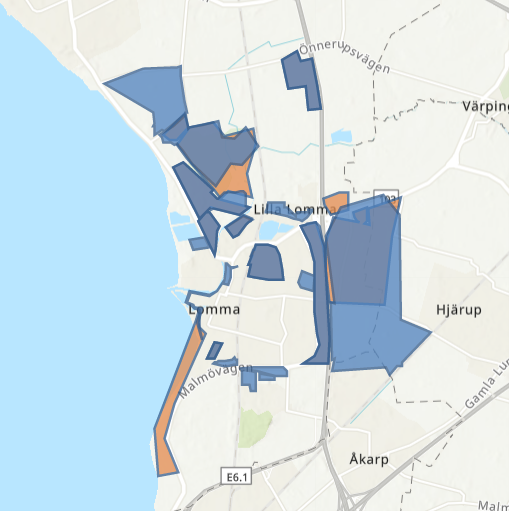
\includegraphics[scale=0.5]{pic4.png}
\label{fig:label}
\end{figure}

\section*{Conclusion}

\bibliographystyle{IEEEtran}
\bibliography{file.bib}



\end{document}
